\documentclass{article}
\usepackage[utf8]{inputenc}
\usepackage[ngerman,english]{babel}
\usepackage[T1]{fontenc}
%\renewcommand{\familydefault}{\rmdefault}

\addtolength{\oddsidemargin}{-0.75in}
\addtolength{\evensidemargin}{-0.75in}
\addtolength{\textwidth}{1.5in}

\addtolength{\topmargin}{-.9in}
\addtolength{\textheight}{1.5in}

\usepackage{amsmath,amssymb}
\usepackage{longtable}
\usepackage{graphicx}
\graphicspath{ {pictures/} }
\usepackage{caption}
\usepackage{subcaption}
\usepackage{adjustbox}
\usepackage{multirow}

\usepackage{titlesec}
\usepackage{anyfontsize}

\usepackage{hyperref}
\hypersetup{
	colorlinks=true,
	linkcolor=black,
	filecolor=black,      
	urlcolor=blue,
}\pagestyle{myheadings}

\usepackage{scrpage2}
\pagestyle{scrheadings}
\clearscrheadfoot

\urlstyle{same}

\graphicspath{ {../data/} {../output/}}

\usepackage[backend=bibtex,style=numeric]{biblatex}
\addbibresource{literature.bib}

 
\begin{document}
\noindent

\section*{Code documentation}

In this code several methods for estimating depth in a stereo image (image \ref{fig:Stereo}) are implemented. For this purpose a \textit{matching cost volume} is calculated by means of sum of squared differences (SSD), sum of absolute differences (SAD) and normalised cross-correlation (NCC) and then the most appropriate match chosen either by the simple \textit{winner-takes-it-all} approach (WTA) or \textit{semi-global matching} (SGM). For this purpose the given images have to be converted to grayscale.

\begin{figure}[!htb]
	\captionsetup[subfigure]{labelformat=empty}
	\centering
	\begin{adjustbox}{minipage=\linewidth,scale=0.95}
		\begin{subfigure}{0.45\textwidth}
			\centering
			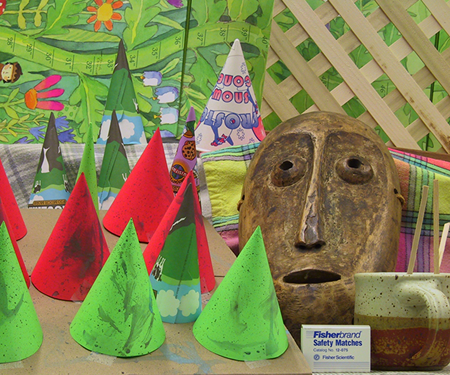
\includegraphics[width=0.9\linewidth]{cones_left.png}
			\caption{a) left}
		\end{subfigure}
		\begin{subfigure}{0.45\textwidth}
			\centering
			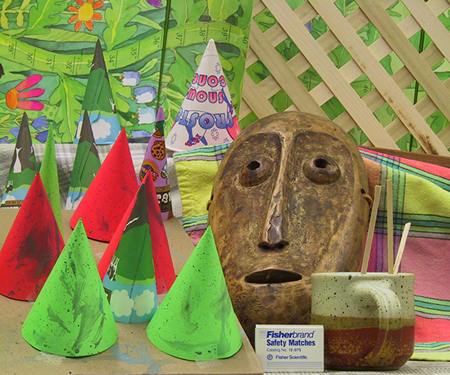
\includegraphics[width=0.9\linewidth]{cones_right.png}
			\caption{b) right}
		\end{subfigure}%
		\par \bigskip
		\begin{subfigure}{0.45\textwidth}
			\centering
			
\includegraphics[width=0.9\linewidth]{cones_gt.png}
			\caption{c) ground-truth}
		\end{subfigure}
		\begin{subfigure}{0.45\textwidth}
			\centering
			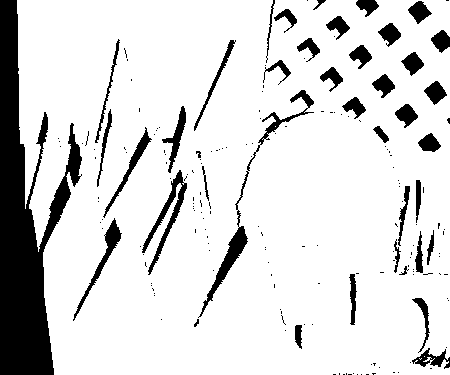
\includegraphics[width=0.9\linewidth]{cones_mask.png}
			\caption{d) mask}
		\end{subfigure}%
	\end{adjustbox}
	\caption[Input]{Stereo images: left (a) and right (b), the corresponding ground-truth (c) and the mask (d) needed for the accX evaluation}
	\label{fig:Stereo}
\end{figure}


\section{Local matching}
The following error-measures and correlations will be used for evaluating a corresponding matching cost between two image patches $p$ and $q$ of equal size $W \times H$.

\subsection{Sum of absolute differences}
In case of the sum of absolute differences the matching of two patches $p$ and $q$ is penalised depending on the sum of absolute differences of the two windows according to
\begin{equation}
SAD(p,q) = \sum\limits_{x=1}^W \sum\limits_{y=1}^H | p(x,y) - q(x,y) |
\end{equation}
This means very similar image patches lead to a low SAD while non-matching patches result in a high SAD.

\subsection{Sum of squared differences}
In case of the sum of squared differences the matching process is penalised quadratically instead of linearly making use of the squared difference instead
\begin{equation}
SSD(p,q) = \sum\limits_{x=1}^W \sum\limits_{y=1}^H ( p(x,y) - q(x,y) )^2
\end{equation}

\subsection{Normalised cross-correlation}
In the case of the more sophisticated normalised cross-correlation the patches are normalised by substracting the means to account for slight deviations in lighting between the two pictures
\begin{equation}
\overline{p} = \frac{1}{H \, W} \sum\limits_{x=1}^W \sum\limits_{y=1}^H p(x,y) \hspace{3cm} \overline{q} = \frac{1}{H \, W} \sum\limits_{x=1}^W \sum\limits_{y=1}^H q(x,y)
\end{equation}
and calculating the a correlation measure for local matching according to
\begin{equation}
NCC(p,q) = \frac{\sum\limits_{x=1}^W \sum\limits_{y=1}^H (p(x,y) - \overline{p}) (q(x,y) - \overline{q})}{\sqrt{\left[ \sum\limits_{x=1}^W \sum\limits_{y=1}^H (p(x,y) - \overline{p})^2 \right] \cdot \left[ \sum\limits_{x=1}^W \sum\limits_{y=1}^H (q(x,y) - \overline{q})^2 \right] }}
\end{equation}
where in this case a high similarity between the two patches contrary to SAD and SSD is characterised by a high NCC. This means for our cost volume we either have to reverse the sign multiplying the $NCC$ by $-1$.

\section{Cost volume}
We use these similarity measures to compute a cost-volume $CV$ for a pre-defined range of disparities $D$
\begin{equation}
CV(x,y,d) = S(I_0(x,y) \, I_1(x - d,y) )
\end{equation}
where the parameter $d \in \mathcal{D}$ and $\mathcal{D} = \left\{ 0, ... \, , D-1 \right\}$ are all valid disparities and $S$ is any of the aforementioned error-measures.

This basically means that we take the left picture and translate the right picture trying to overlap the objects in the two pictures taken from different views. The points at a certain depth have a certain disparity and thus the optimal shift can be used to determine the correct depth. In order to account for a certain deviation we use a certain search window $(W,H)$ rather than trying to match the points directly.

\section{Matching algorithm}

\subsection{Winner-takes-it-all solution}
One fast way of obtaining then the best disparity for each image point would be taking the point with the highest value in the cost volume along the disparity axis according to
\begin{equation}
\overline{d}(x,y) \in \arg \min_d CV(x,y,d)
\end{equation}
This though leads to noisy results as this approach doesn't penalise label changes at all.

\subsection{Semi-global matching}

In semi-global matching a different approach is taken, rather than looking for the best fit on a scanline, a sort of global optimisation is used. Each pixel with a corresponding unary cost given by the cost volume is assigned an additional pairwise cost that depends on wherever the neighbouring pixels have a similar depth value or deviate significantly. This energy can be written as
\begin{equation}
\min_z \left[ \sum_{i \in \mathcal{V}} g_i (z_i) + \sum_{(i,j) \in \mathcal{E}} f_{i,j} (z_i, z_j) \right]
\end{equation}
where $\mathcal{V}$ are the image pixels, $\mathcal{E}$ the edges, the connections between two pixels. The $g_i$ are given by the cost volume and the pairwise cost $f_{i,j}$ defines a penalty for jumps between neighbouring pixels.
\begin{equation}
f_{i,j} (z_i, z_j) = \begin{cases}
0, \hspace{0.7cm} \text{if} \, z_i = z_j \\
L_1, \hspace{0.5cm} \text{if} \, |z_i - z_j| = 1\\
L_2\phantom{,} \hspace{0.5cm} \text{else}
\end{cases}
\end{equation}
This is done as following: First messages for all four disparity directions are calculated where the first message in each direction is initialised with $\vec 0$.
\begin{equation}
m_{i+1}^a(t) = \min_{s \in \mathcal{D}} \left[ m_i^a(s) + f_{i, i+1} (s,t) + g_i(s) \right]
\end{equation}
This can be done for every direction by a combination of mirroring and transposing the cost volume. Then the beliefs are computed
\begin{equation}
b_i(s) = g_i(s) \sum_{a \in \{ L,R,U,D \}} m_i^a(s)
\end{equation}
The correct disparity is then calculated from the believes as follows
\begin{equation}
\hat{d} (x,y) \in \arg \min_d b(x,y,d)
\end{equation}
The last formula contains is intentionally given as $\in$ as the solutions might not be unique.

\section{Evaluation: compare to ground-truth}
The performance of the stereo workflow is evaluated by comparing it with a ground-truth disparity map, in this case with the $accX$ measure
\begin{equation}
accX(z,z*) = \frac{1}{Z} \sum\limits_{x=1}^W \sum\limits_{y=1}^H m(x,y) \cdot \begin{cases}
1, \hspace{0.5cm} \text{if} \, |(z(x,y) - z*(x,y)| \leq X\\
0\phantom{,} \hspace{0.5cm} \text{else}
\end{cases}
\end{equation}
This measure characterises errors less than or equal to $X$ disparities, between the prediction $z$ and the ground truth disparity map $z*$ with a mask $m$ that contains $1$ for the $Z$ valid pixels and $0$ for the invalid pixels.

The mask basically excludes pixels that should not be evaluated e.g. because they are occluded in either of the two pictures. The average of the remaining pixels that were estimated correctly is determined. All pixels that guessed the depth correctly (threshold $X$) are set to $1$, all pixels that did not estimate it correctly do not contribute. In this way the $accX$ measures the amount of pixels that were matched correctly to those that could possibly be matched. An $accX$ of 1 would correspond to the ground truth.

\end{document}